
\documentclass[a4paper,12pt]{article}
\usepackage{enumitem} % -> Alphabetical Lists
\usepackage{amsmath} % -> Matrices
\usepackage{fullpage} % -> A4 Full Page
\usepackage{amssymb} % -> Therefore
\usepackage[utf8]{inputenc}
\usepackage{graphicx}
\usepackage{adjustbox}
\usepackage{listings}
\usepackage{braket}
\usepackage{geometry}
\usepackage{tikz}
\usepackage{gensymb}

\usetikzlibrary{quantikz}

\graphicspath{ {./} }

\geometry{
    a4paper,
    total={170mm,257mm},
    left=20mm,
    top=20mm,
}

\title{Quantum Computing Assignment 6 - Group 18}
\author{
    Rallabhandi, Anand Krishna 
    \and
    Mustafa, Syed Husain
    \and
     , Mohammed Kamran 
}
\date{\today}

\begin{document}

\maketitle

\section*{Exercise 6.1}

 \begin{large}(\textbf{Two bit Quantum Search})
 \end{large}

\begin{enumerate}[label=(\alph*)]
    \item \phantom{-} \\
    \begin{center}
        \begin{quantikz}
            \lstick{$\ket{x}$} & \qw & \gate{X} & \qw & \ctrl{1} & \qw & \gate{X} & \qw \\
            \lstick{$\ket{y}$} & \qw  &\gate{X} &\gate{H} & \targ{} & \gate{H} &\gate{X} &\qw
        \end{quantikz}
    \end{center}
    We're given the negated phase gate appearing in the Grover Operator, ie; $-2(\ket{00}\bra{00}-I)$ \\
    This term can be expanded into matrix form as follows : 
    \[-2\begin{pmatrix}
        1 \\
        0 \\
        0 \\
        0 \\
    \end{pmatrix}_{4 \times 1} \times \hspace{3mm}\begin{pmatrix}
        1 & 0 & 0 & 0 \\
    \end{pmatrix}_{1 \times 4} \hspace{3mm}-\hspace{3mm} \begin{pmatrix}
        1 & 0 & 0 & 0 \\
        0 & 1 & 0 & 0 \\
        0 & 0 & 1 & 0 \\
        0 & 0 & 0 & 1 \\
    \end{pmatrix}_{4 \times 4} = \begin{pmatrix}
        -1 & 0 & 0 & 0 \\
        \phantom{-}0 & 1 & 0 & 0\\
        \phantom{-}0 & 0 & 1 & 0 \\
        \phantom{-}0 & 0 & 0 & 1\\
    \end{pmatrix}_{4 \times 4} \hspace{22mm} \textbf{(A)}\]
    Implementing the above circuit on some arbitrary states $\ket{x}$ \& $\ket{y}$. \\
    Consider $\ket{x} = 0 $ \& $\ket{y} = 0$: 
    \[\ket{00} \xrightarrow{\text{$X \otimes X$}}\ket{11} \xrightarrow{\text{$I \otimes H$}} \ket{1}\Big( \frac{\ket{0}-\ket{1}}{\sqrt{2}}\Big) \xrightarrow{\text{CNOT}}\ket{0}\Big(\frac{\ket{1}-\ket{0}}{\sqrt{2}}\Big)\xrightarrow{\text{$I \otimes H$}}-\ket{11} \xrightarrow{\text{$X \otimes X$}}-\ket{00} \hspace{5mm}\textbf{(B)}\]
    Consider $\ket{x} = 0 $ \& $\ket{y} = 1$: 
    \[\ket{01} \xrightarrow{\text{$X \otimes X$}}\ket{10} \xrightarrow{\text{$I \otimes H$}} \ket{1}\Big( \frac{\ket{0}+\ket{1}}{\sqrt{2}}\Big) \xrightarrow{\text{CNOT}}\ket{1}\Big(\frac{\ket{1}+\ket{0}}{\sqrt{2}}\Big)\xrightarrow{\text{$I \otimes H$}}\ket{10} \xrightarrow{\text{$X \otimes X$}}\ket{01}\hspace{13mm}\textbf{(C)}\]
    Consider $\ket{x} = 1 $ \& $\ket{y} = 0$: 
    \[\ket{10} \xrightarrow{\text{$X \otimes X$}}\ket{01} \xrightarrow{\text{$I \otimes H$}} \ket{0}\Big( \frac{\ket{0}-\ket{1}}{\sqrt{2}}\Big) \xrightarrow{\text{CNOT}}\ket{0}\Big(\frac{\ket{0}-\ket{1}}{\sqrt{2}}\Big)\xrightarrow{\text{$I \otimes H$}}\ket{01} \xrightarrow{\text{$X \otimes X$}}\ket{10}\hspace{13mm}\textbf{(D)}\]
    Consider $\ket{x} = 1 $ \& $\ket{y} = 1$: 
    \[\ket{11} \xrightarrow{\text{$X \otimes X$}}\ket{00} \xrightarrow{\text{$I \otimes H$}} \ket{0}\Big( \frac{\ket{0}+\ket{1}}{\sqrt{2}}\Big) \xrightarrow{\text{CNOT}}\ket{0}\Big(\frac{\ket{0}+\ket{1}}{\sqrt{2}}\Big)\xrightarrow{\text{$I \otimes H$}}\ket{00} \xrightarrow{\text{$X \otimes X$}}\ket{11}\hspace{13mm}\textbf{(E)}\]
    The four results \textbf{(B)}, \textbf{(C)}, \textbf{(D)}, \& \textbf{(E)} are the column vectors of the result \textbf{(A)} \\
    \begin{center}
        $\therefore$ The result of the above circuit is equivalent to the negated phase gate appearing in the Grover Operator
    \end{center}
    \item \phantom{-} \\
    Given M = 1, N = 4, \& $\sin\big(\frac{\theta}{2}\big)=\sqrt{\frac{M}{N}}$\\~\\
    $\implies \frac{\theta}{2} = \sin^{-1}\Big(\sqrt{\frac{1}{4}}\Big) \implies \frac{\theta}{2} = \sin^{-1}\Big(\pm\frac{1}{2}\Big) \implies \frac{\theta}{2} = 30\degree \implies \theta = 60\degree $  \\~\\
    Given $G^{k}\ket{\psi} = \cos\Big(\big(\frac{1}{2}+k\big)\theta\Big)\ket{\alpha} + \sin\Big(\big(\frac{1}{2}+k\big)\theta\Big)\ket{\beta}$ \\~\\
    Consider single application of Grover's Operator, i.e; k=1. \\~\\
    $\implies G\ket{\psi} = \cos\Big(\frac{3}{2}\theta\Big)\ket{\alpha}+\sin\Big(\frac{3}{2}\theta\Big)\ket{\beta} \implies G\ket{\psi} = \cos(90\degree)\ket{\alpha}+\sin(90\degree)\ket{\beta}\\ \implies G\ket{\psi} = \ket{\beta}$

    \item \phantom{-} \\  
    \graphicspath{./images/}
    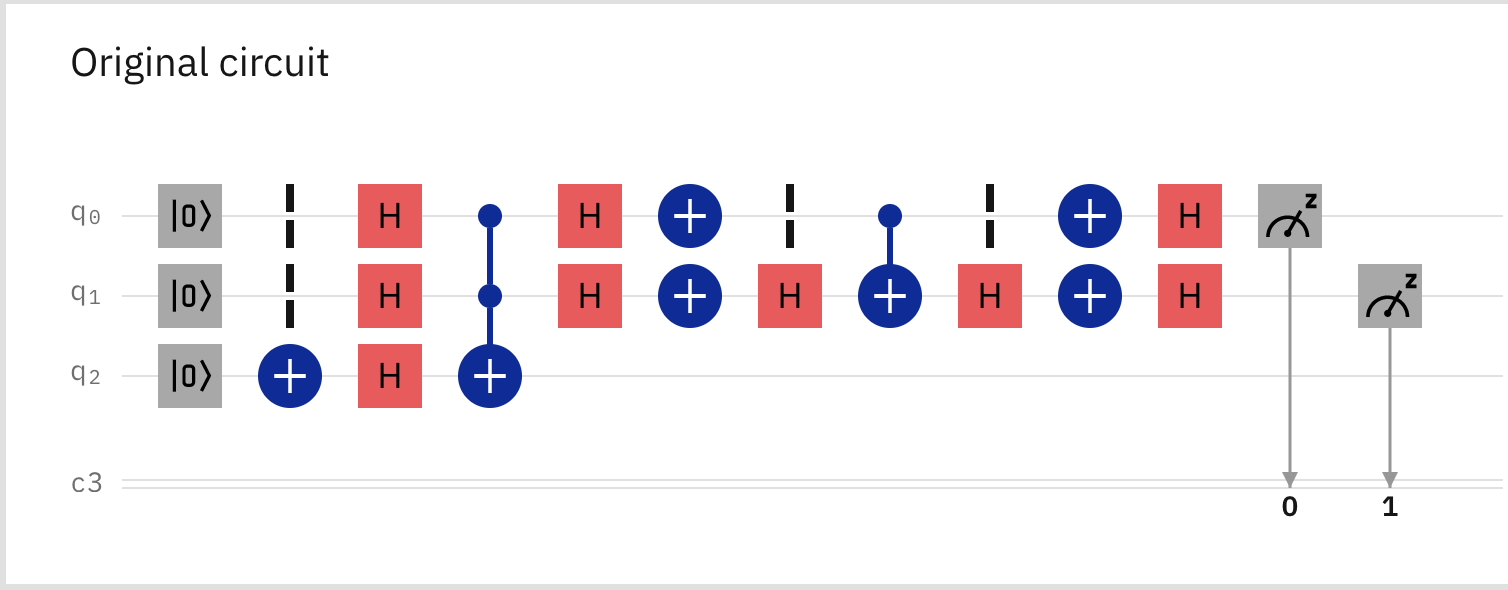
\includegraphics[scale=0.40]{images/im1.png}\\
    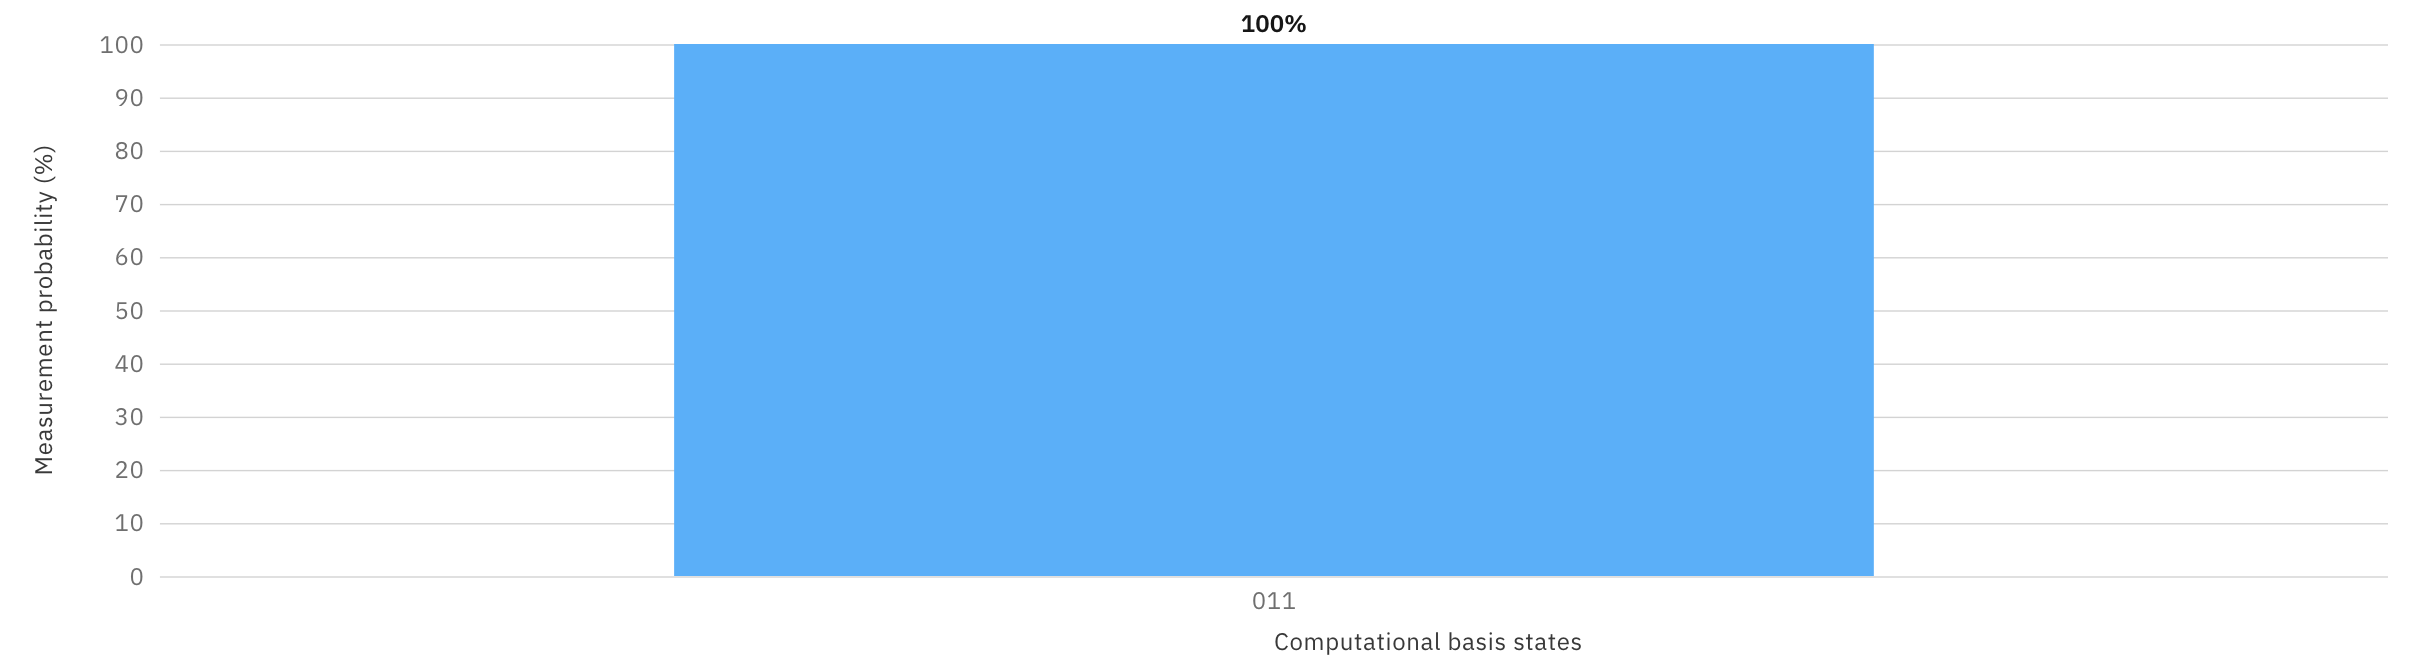
\includegraphics[scale=0.40]{images/im2.png}
    
\end{enumerate}

\section*{Exercise 6.2}

 \begin{large}(\textbf{Bloch Sphere for mixed-state qubits})
\end{large}
\begin{enumerate}[label=(\alph*)]
    
    \item \phantom{-} \\A density matrix is hermitian, thus 

    \begin{gather*}
     \rho =   \begin{bmatrix}
     a & b*\\
    b* & d
    \end{bmatrix}
    a=\frac{1+v_3}{2}, d = \frac{1-v_3}{2} , b = \frac{v_1-i*v_2}{2}
    \\~\\
    \rho =  \frac{1}{2} *  \begin{bmatrix}
     1+v_3 & v_1-i*v_2\\
    v_1+i*v_2 & 1-v_3 
    \end{bmatrix} = \frac{I + r.\sigma}{2}\\
    \end{gather*}
    Computing eigenvalues of this matrix, we get\\
    \begin{gather*}
    det = ( \frac{1}{2} * \begin{vmatrix}
     v_3+1-\lambda & v_1 -i*v_2\\
    v1+i*v_2 & -v_3 + 1 - \lambda 
    \end{vmatrix})
    \\~\\
    \frac{1}{2}*[(1-\lambda)^2 - (v_3)^2 - v_1^2 - v_2^2] = 0 \\~\\
    \lambda = 1 \pm \sqrt{v_1^2 + v_2^2 + v_3^3}\\~\\
    \lambda = 1 \pm |r|
    \end{gather*}
    Since $\rho$ is Positive, we get 
    \begin{gather*}
        1 - |r| >=0 \\~\\
        |r| <=1
    \end{gather*}\\~\\
    Thus an arbitary density matrix  $\rho$ in a mixed state can be written in the form 
    \begin{gather*}
       \rho = \frac{I + r.\sigma}{2}\\ 
    \end{gather*}
    \item \phantom{-} \\
    
Since state $\rho$ is pure, we get
\begin{gather*}
tr[\rho^2]=1\\~\\
tr[\frac{I + r.\sigma}{2} * \frac{I + r.\sigma}{2}] = 1\\~\\
tr[\frac{1}{4} *  \begin{bmatrix}
1+v_3 & v_1-i*v_2\\
v_1+i*v_2 & 1-v_3
\end{bmatrix} * \begin{bmatrix}
1+v_3 & v_1-i*v_2\\
v_1+i*v_2 & 1-v_3
\end{bmatrix}] = 1\\~\\
\frac{1}{4} * [(1 +v_3)^2 + 2(v_1^2 + v_2^2) +(1 -v_3)^2] =1\\~\\
2 + 2(v_1^2 + v_2^2 + v_3*2) = 4 \\
|r|^2 = 1\\~\\
|r|=1
\end{gather*}
Thus a state is pure if and only if $|r|=1$
    
\item \phantom{-} \\ 
    For a pure state $\ket{\psi}$ we know that the density opertor is given by $\rho = \ket{\psi}\bra{\psi}$.\\
    Consider $\ket{\psi} = e^{i\gamma}\Big(\cos\big(\frac{\theta}{2}\big)\ket{0} + e^{i\varphi}\sin\big(\frac{\theta}{2}\big)\ket{1}\Big)$ . \\We compute $\ket{\psi}\bra{\psi}$ as follows:\\
    $\ket{\psi}\bra{\psi} = e^{i\gamma}\begin{pmatrix}
        \cos\big(\frac{\theta}{2}\big) \\
        e^{i\varphi}\sin\big(\frac{\theta}{2}\big) 
    \end{pmatrix} \times e^{i\gamma}\begin{pmatrix}
        \cos\big(\frac{\theta}{2}\big) & e^{-i\varphi}\sin\big(\frac{\theta}{2}\big)
    \end{pmatrix} \\ \implies \ket{\psi}\bra{\psi} = e^{2i\gamma}\begin{pmatrix}
        cos^{2}\big(\frac{\theta}{2}\big) & e^{-i\varphi}\cos\big(\frac{\theta}{2}\big)\sin\big(\frac{\theta}{2}\big) \\
        e^{i\varphi}\cos\big(\frac{\theta}{2}\big)\sin\big(\frac{\theta}{2}\big) & sin^{2}\big(\frac{\theta}{2}\big)

    \end{pmatrix}$ \\
    $\implies \ket{\psi}\bra{\psi} = \begin{pmatrix}
        1 + \cos(\theta) & e^{-i\varphi}\sin(\theta) \\
        e^{i\varphi}\sin(\theta) & 1-\cos(\theta) \\
    \end{pmatrix} \hspace{35mm} \textbf{(A)}$ \\~\\The phase term is inconsequential hence removed. \\~\\
    We applied the following trigonometric properties to obtain  \textbf{(A)}. \\~\\
    $\sin(\theta) = 2\sin(\frac{\theta}{2})\cos(\frac{\theta}{2}), \hspace{5mm} 1+cos(\theta) = \cos^{2}(\frac{\theta}{2}),\hspace{1mm} \text{and} \hspace{5mm} 1-\cos(\theta) = \sin^{2}(\frac{\theta}{2})$ \\~\\
    Consider $\rho = \frac{1}{2}\Big(1+r\sigma\Big) \implies \rho = \begin{pmatrix}
        1 + r_{3} & r_{1}-ir_{2} \\
        r_{1}+ir_{2} & 1 - r_{3} \\
    \end{pmatrix} \hspace{9mm} \textbf{(B)}$ \\~\\
    Comparing \textbf{(A)} \& \textbf{(B)} $\implies r = \begin{pmatrix}
        sin(\theta)cos(\varphi) \\
        sin(\theta)sin(\varphi) \\
        cos(\theta) \\
    \end{pmatrix}$ \\~\\
    $|r| = \sqrt{\sin^{2}(\theta)\cos^{2}(\varphi) + \sin^{2}(\theta)\sin^{2}(\varphi) +cos^{2}(\theta) } = 1$  \\~\\
    Hence $r$ coincides with $\ket{\psi}$ on the Bloch Sphere.
    

\end{enumerate}

\end{document}
